% ==============================================
\section{Introduction}
\label{sec:intro}
% ==============================================

\begin{figure}
\centering
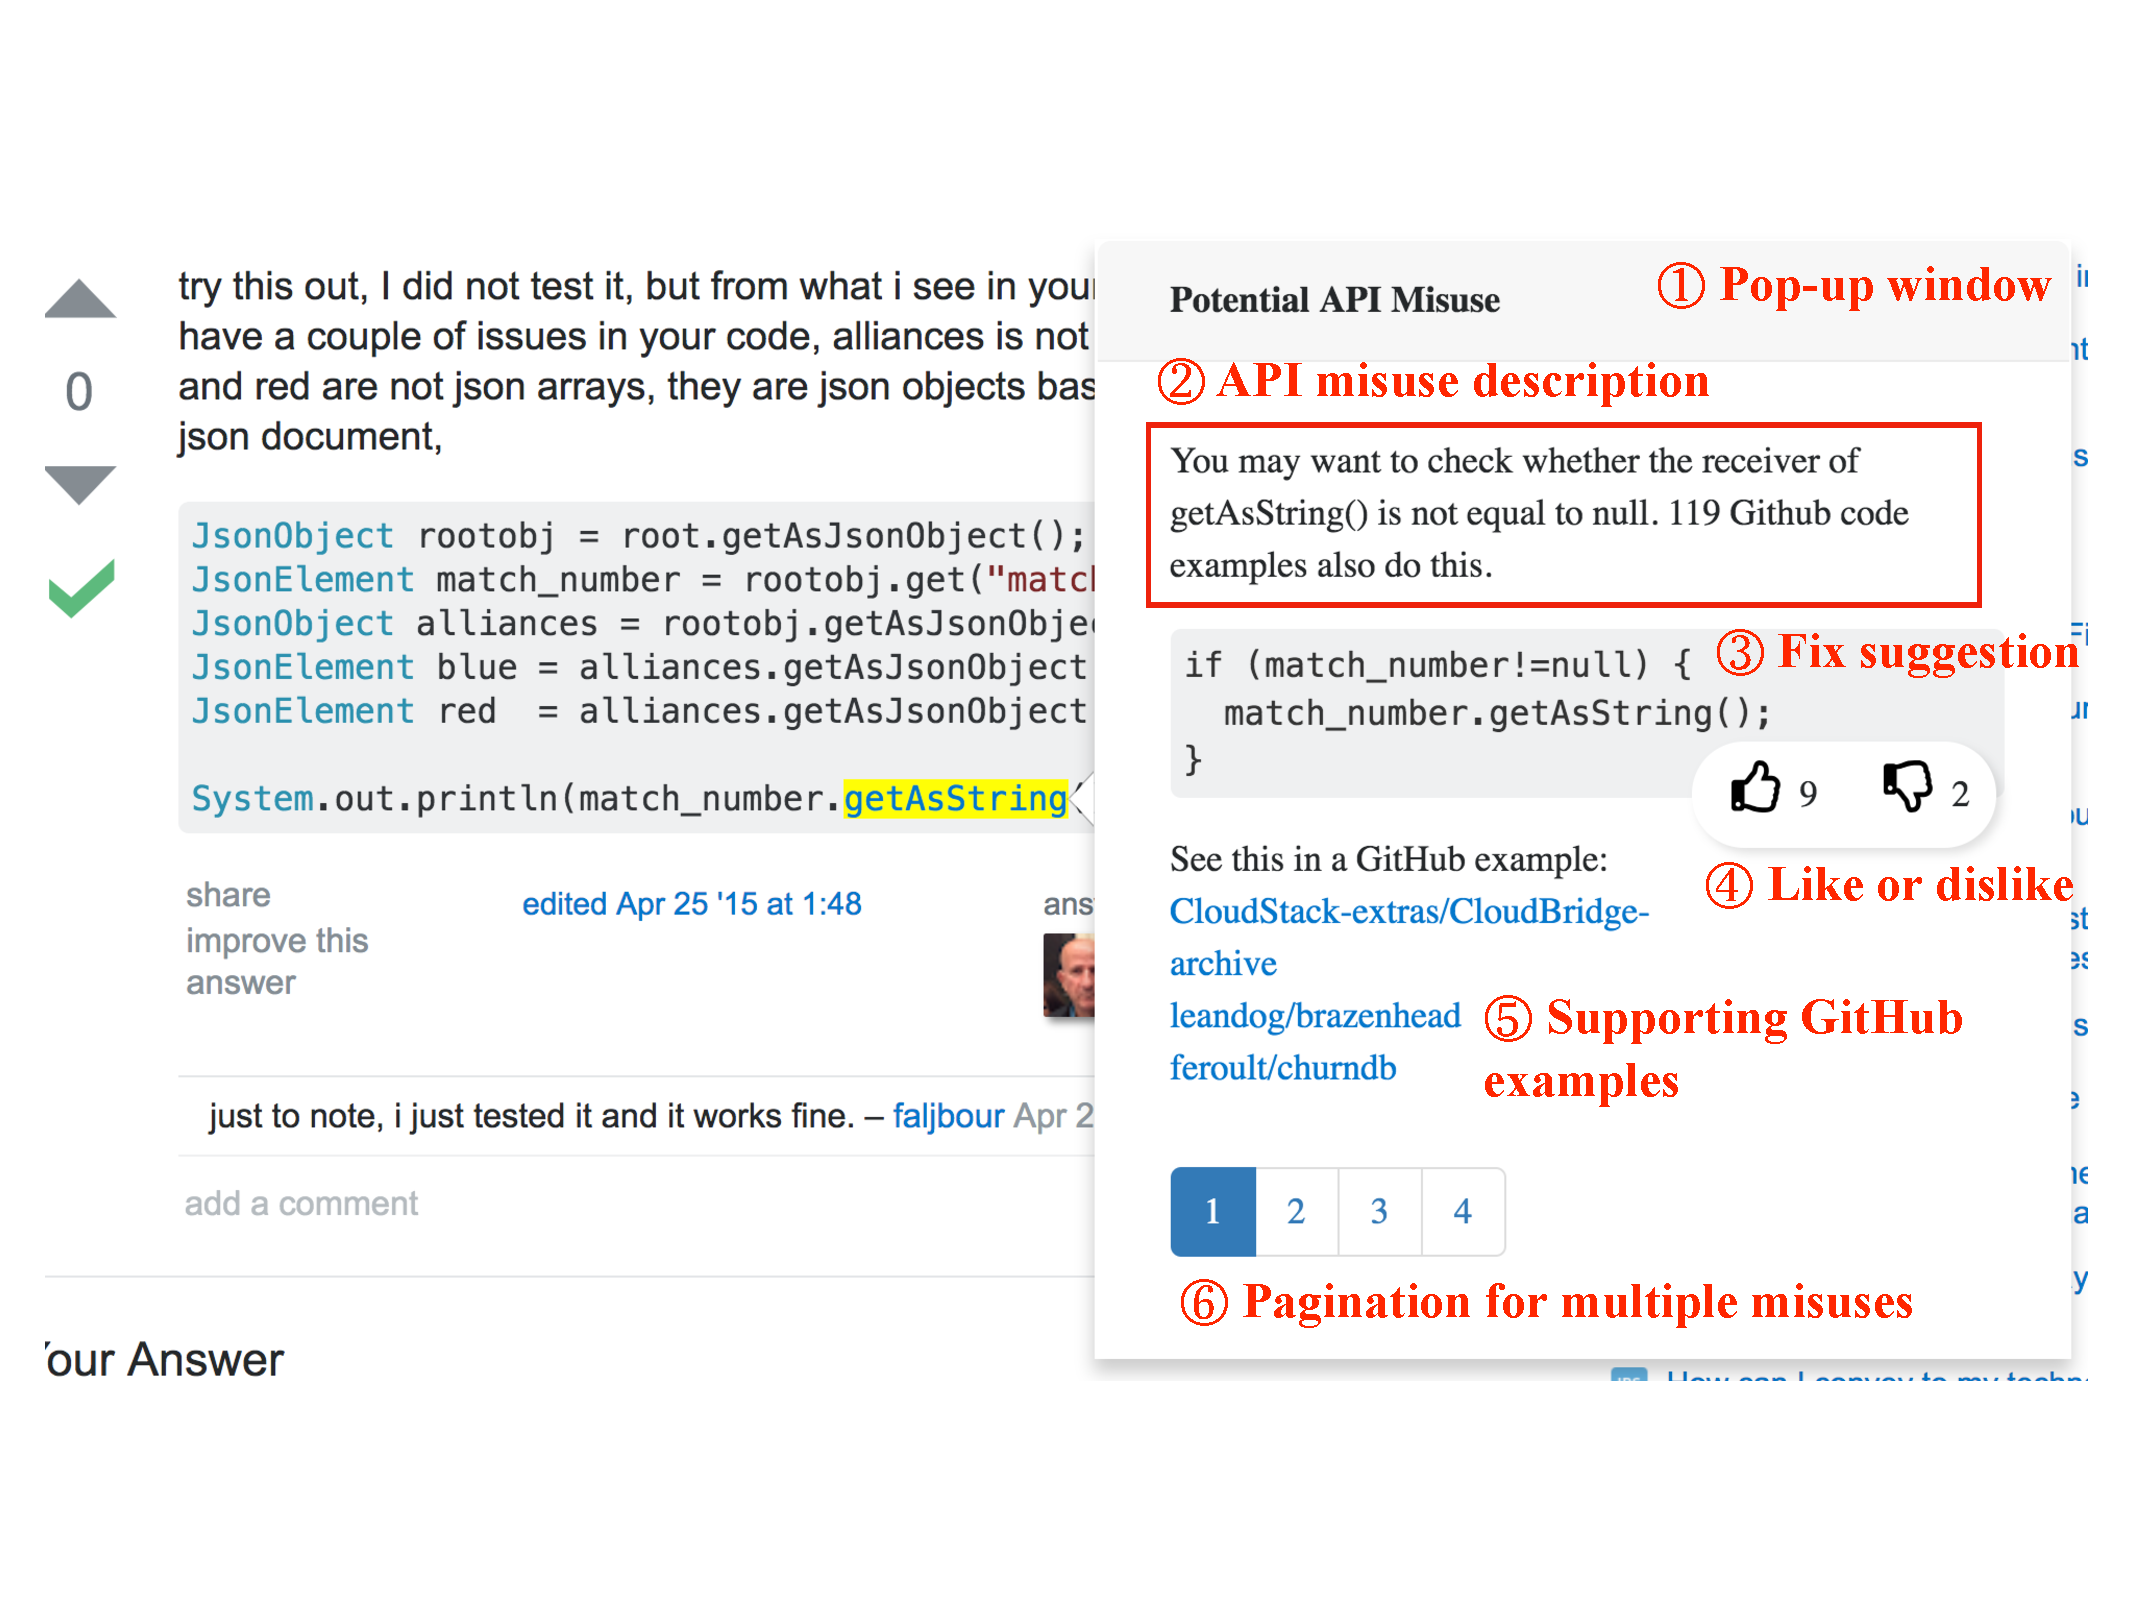
\includegraphics[width=0.5\textwidth]{examplecheck-screenshot.pdf}
  \caption{The {\tool} Chrome extension that augments Stack Overflow with API misuse warnings. The pop-up window alerts that {\ttt match\_number} can be {\ttt null} if the requested {\ttt JSON} attribute does not exist and will crash the program by throwing {\ttt NullPointerException} when {\ttt getAsString} is called on it.}
  \label{fig:screenshot}
  \vspace{-0.1in}
\end{figure}

% Problem
Programmers often search for online code examples to learn new APIs. A case study at Google shows that developers issue an average of 12 code search queries per weekday~\cite{sadowski2015developers}. Stack Overflow (SO) is a popular Q\&A website that programmers often resort to. As of July 2017, Stack Overflow has accumulated more than 22 million answers, many of which contain code snippets for specific programming questions. However, SO snippets are not always complete or reliable, which can be misleading and sometimes harmful when programmers follow them {\em as-is} during software development. For example, Fischer et al.~found that 29\% of security-related code snippets in Stack Overflow were insecure and might affect over 1 million Android apps in Google play~\cite{fischer2017stack}. 

% Solution
This paper presents {\tool}, a Chrome extension that informs programmers about API usage violations in Stack Overflow posts. Figure~\ref{fig:screenshot} shows a screenshot of {\tool}. To detect API usage violations, {\tool} contrasts SO snippets with API usage patterns mined from 380K GitHub repositories. The mining technique is detailed in our ICSE 2018 paper~\cite{zhang2018code}. These patterns abstract away syntactic details such as variable names, but retain the temporal ordering, control structures, and guard conditions of API calls. Our insight is that common API usage from a large corpus may represent a desirable pattern that a programmer can use to examine and enhance SO code snippets. 

Given a SO post, {\tool} first extracts the sequence of API calls with corresponding control constructs and guard conditions. {\tool} then contrasts the call sequence with corresponding patterns learned from GitHub and highlights method calls that violate the common usage patterns. To help users better understand a detected violation, {\tool} generates a descriptive warning message and also illustrates how to fix the violation. {\tool} quantifies how many GitHub developers also follow the same pattern and provides some samples of supporting GitHub examples. However, using common API usage patterns to detect violations may lead to false alarms, since these patterns do not represent infrequent but correct API usage scenarios. To mitigate this issue, {\tool} allows users to upvote or downvote a violation based on its applicability and usefulness to a SO post. 

This tool demonstration paper focuses on the tool features and implementation details of the Chrome extension. Our previous paper~\cite{zhang2018code} describes the API usage mining technique and the empirical findings in Stack Overflow, which motivates the design of the Chrome extension. The manual inspection of 400 Stack Overflow posts with API usage violations detected by {\tool} is also presented in~\cite{zhang2018code}. 

%By examining 217K SO posts with the validated patterns, we found that 31\% of SO posts might have potential API usage violations, which could produce symptoms such as program crashes and resource leaks. This empirical finding motivates the design and implementation of the Chrome extension, which is the main contribution of this paper. Both the dataset of API usage patterns and the SO posts with potential API usage violations are available for download at {\small{\url{http://web.cs.ucla.edu/~tianyi.zhang/examplecheck.html}}}.


%A user of {\tool} would benefit from the addition of concrete examples from the production code in GitHub, when inspecting or reusing code snippets in Stack Overflow. This will not only combat programming issues stemming from the use of incomplete or unreliable SO code snippets, but will also be an aid for users learning a new API. 

%A user of this tool would benefit from not needing to cross-reference multiple sites for proper API usage reference, and will be able to continue using Stack Overflow to learn APIs with the added advantage of seeing which usage patterns a post may have left out of its explanation. This could result in more complete, reliable code with minimal added time or effort on the part of the programmer.\todo{The description here does not sound very appealing. Can you rework this paragraph?} 

%input{fig_motiExample}
%\input{fig_UI}
